\documentclass[english,,man]{apa6}
\usepackage{lmodern}
\usepackage{amssymb,amsmath}
\usepackage{ifxetex,ifluatex}
\usepackage{fixltx2e} % provides \textsubscript
\ifnum 0\ifxetex 1\fi\ifluatex 1\fi=0 % if pdftex
  \usepackage[T1]{fontenc}
  \usepackage[utf8]{inputenc}
\else % if luatex or xelatex
  \ifxetex
    \usepackage{mathspec}
  \else
    \usepackage{fontspec}
  \fi
  \defaultfontfeatures{Ligatures=TeX,Scale=MatchLowercase}
\fi
% use upquote if available, for straight quotes in verbatim environments
\IfFileExists{upquote.sty}{\usepackage{upquote}}{}
% use microtype if available
\IfFileExists{microtype.sty}{%
\usepackage{microtype}
\UseMicrotypeSet[protrusion]{basicmath} % disable protrusion for tt fonts
}{}
\usepackage{hyperref}
\hypersetup{unicode=true,
            pdftitle={The Unsung Principles of Dynamics},
            pdfauthor={Christopher R. Dishop, Jeffrey Olenick, \& Richard. P DeShon},
            pdfkeywords={\ldots{}.},
            pdfborder={0 0 0},
            breaklinks=true}
\urlstyle{same}  % don't use monospace font for urls
\ifnum 0\ifxetex 1\fi\ifluatex 1\fi=0 % if pdftex
  \usepackage[shorthands=off,main=english]{babel}
\else
  \usepackage{polyglossia}
  \setmainlanguage[]{english}
\fi
\usepackage{graphicx,grffile}
\makeatletter
\def\maxwidth{\ifdim\Gin@nat@width>\linewidth\linewidth\else\Gin@nat@width\fi}
\def\maxheight{\ifdim\Gin@nat@height>\textheight\textheight\else\Gin@nat@height\fi}
\makeatother
% Scale images if necessary, so that they will not overflow the page
% margins by default, and it is still possible to overwrite the defaults
% using explicit options in \includegraphics[width, height, ...]{}
\setkeys{Gin}{width=\maxwidth,height=\maxheight,keepaspectratio}
\IfFileExists{parskip.sty}{%
\usepackage{parskip}
}{% else
\setlength{\parindent}{0pt}
\setlength{\parskip}{6pt plus 2pt minus 1pt}
}
\setlength{\emergencystretch}{3em}  % prevent overfull lines
\providecommand{\tightlist}{%
  \setlength{\itemsep}{0pt}\setlength{\parskip}{0pt}}
\setcounter{secnumdepth}{0}
% Redefines (sub)paragraphs to behave more like sections
\ifx\paragraph\undefined\else
\let\oldparagraph\paragraph
\renewcommand{\paragraph}[1]{\oldparagraph{#1}\mbox{}}
\fi
\ifx\subparagraph\undefined\else
\let\oldsubparagraph\subparagraph
\renewcommand{\subparagraph}[1]{\oldsubparagraph{#1}\mbox{}}
\fi

%%% Use protect on footnotes to avoid problems with footnotes in titles
\let\rmarkdownfootnote\footnote%
\def\footnote{\protect\rmarkdownfootnote}


  \title{The Unsung Principles of Dynamics}
    \author{Christopher R. Dishop\textsuperscript{1}, Jeffrey
Olenick\textsuperscript{1}, \& Richard. P DeShon\textsuperscript{1}}
    \date{}
  
\shorttitle{DYNAMICS PRINCIPLES}
\affiliation{
\vspace{0.5cm}
\textsuperscript{1} Michigan State University}
\keywords{....\newline\indent Word count: 95}
\usepackage{csquotes}
\usepackage{upgreek}
\captionsetup{font=singlespacing,justification=justified}

\usepackage{longtable}
\usepackage{lscape}
\usepackage{multirow}
\usepackage{tabularx}
\usepackage[flushleft]{threeparttable}
\usepackage{threeparttablex}

\newenvironment{lltable}{\begin{landscape}\begin{center}\begin{ThreePartTable}}{\end{ThreePartTable}\end{center}\end{landscape}}

\makeatletter
\newcommand\LastLTentrywidth{1em}
\newlength\longtablewidth
\setlength{\longtablewidth}{1in}
\newcommand{\getlongtablewidth}{\begingroup \ifcsname LT@\roman{LT@tables}\endcsname \global\longtablewidth=0pt \renewcommand{\LT@entry}[2]{\global\advance\longtablewidth by ##2\relax\gdef\LastLTentrywidth{##2}}\@nameuse{LT@\roman{LT@tables}} \fi \endgroup}


\DeclareDelayedFloatFlavor{ThreePartTable}{table}
\DeclareDelayedFloatFlavor{lltable}{table}
\DeclareDelayedFloatFlavor*{longtable}{table}
\makeatletter
\renewcommand{\efloat@iwrite}[1]{\immediate\expandafter\protected@write\csname efloat@post#1\endcsname{}}
\makeatother
\usepackage{lineno}

\linenumbers

\authornote{\ldots{}.

Correspondence concerning this article should be addressed to
Christopher R. Dishop, 316 Physics Rd, Psychology Building Room 348,
East Lansing, MI 48823. E-mail:
\href{mailto:dishopch@msu.edu}{\nolinkurl{dishopch@msu.edu}}}

\abstract{
Begin here\ldots{}


}

\usepackage{amsthm}
\newtheorem{theorem}{Theorem}[section]
\newtheorem{lemma}{Lemma}[section]
\theoremstyle{definition}
\newtheorem{definition}{Definition}[section]
\newtheorem{corollary}{Corollary}[section]
\newtheorem{proposition}{Proposition}[section]
\theoremstyle{definition}
\newtheorem{example}{Example}[section]
\theoremstyle{definition}
\newtheorem{exercise}{Exercise}[section]
\theoremstyle{remark}
\newtheorem*{remark}{Remark}
\newtheorem*{solution}{Solution}
\begin{document}
\maketitle

Think about how common it is to find phrases about dynamics scattered
throughout an introduction to an article, phrases like \enquote{we are
going to address the dynamics,} \enquote{taking a dynamic perspective,}
\enquote{prior research has not appreciated the dynamics,} \enquote{we
consider the phenomenon as dynamic,} or \enquote{we examine it on a
dynamic basis.} What do these mean? How do researchers take a dynamic
perspective?

We have noticed a pattern in how people think about and describe
dynamics in empirical studies. Researchers tend to study and convey
their dynamic process of interest with respect to a statistical model or
class of models. For example, researchers that are familiar with growth
models will talk about the importance of growth in a variable or how
within-person trajectories have been ignored in prior research, they
will then estimate a growth curve, and ultimately convey something about
trends or growth over time and how this has added a new dynamic
perspective to our understanding. \enquote{Growth model thinking,} as
well as other recent ways of discussing how things happen over time,
have produced wonderful insights into important processes in
organizational science, and we see them as initial steps toward
dynamics.

When researchers couch their thinking in a model, however, some concepts
naturally go unnoticed. We are accumulating tremendous knowledge by
collecting longitudinal data, focusing on how things happen over time,
and opening the door of dynamics, but there are dynamic principles that
have yet to be exposed in our literature -- we have not yet stepped
fully through the door. In this paper we discuss a variety of dynamics
principles; some are concepts that will reorient how researchers think
about dynamics, and others are statistical properties that, if ignored,
result in biased inferences. Ultimately we are bringing attention to
principles that should be incorporated if we are truly interested in a
\enquote{dynamic perspective.}

Below, we first discuss two broad classes of \enquote{thinking with
respect to a statistical model} that have done the hard work -- they are
sets of empirical studies taking initial steps towards dynamics. The
first we call \enquote{growth,} and the second \enquote{relationships,}
and we discuss example studies in each to briefly show our field's
interest in dynamics and how some researchers approach it. These first
two sections are not exhaustive, we are simply sampling a few of the
common ways researchers currently think about dynamics to motivate the
core of the paper. There, we unpack the dynamic principles.

\hypertarget{stepping-toward-dynamics-growth}{%
\section{Stepping Toward Dynamics --
Growth}\label{stepping-toward-dynamics-growth}}

One of the first steps our field is taking toward appreciating dynamics
is by examining whether something goes up or down over time -- examining
trend or \enquote{growth} patterns.

Hülsheger (2016) explores fatigue trends. He motivates his study by
stating that his examination of the \enquote{the continuous ebb and flow
of fatigue over the course of the day and about the factors that
influence this temporal ebb and flow} responds to calls to
\enquote{empirically address the dynamic process of recovery and thereby
helps refine recovery theory} (p.~906). For 5 consecutive workdays he
assesses fatigue with self-report surveys -- one in the morning, another
at the first work break, a third at the end of work, and the last in the
evening -- among a sample of Dutch employees. All surveys measure
fatigue, and the morning survey also assessses sleep quality whereas the
fourth measures psychological detachment. He estimates fatigue growth
curves and correlates sleep quality and psychological detachment with
both the fatigue intercept and slope, respectively.

Dunford, Shipp, Boss, Angermeier, and Boss (2012) examine burnout
trajectories over two years. They motivate their study by stating that,
\enquote{theoretically, much of the burnout literature suggests that
burnout should be progressive and dynamic, yet most empirical research
has focused on explaining and testing the antecedents of static levels
of burnout,} therefore \enquote{knowing for whom burnout changes and
when this pattern of change occurs leads to a more realistic view of the
dynamism of human experience and better managerial prescriptions for
addressing burnout} (p.~637). Over two years they assess healthcare
workers with five measurements, each separated by six months. All
surveys measure burnout (all dimensions), and the researchers also
collect between person assessments of job transitions (a categorical
variable indicating whether an employee is a newcomer, recently
underwent an internal job change, or remained at the same position
throughout). They estimate a sequence of growth curves and examine
linear and quadratic slope terms for all three burnout dimensions. They
also covary job transition type with the intercept and slope terms.

\hypertarget{summary}{%
\subsection{Summary}\label{summary}}

These authors are clearly interested in dynamics, and in this framework
they examine within-person trajectories, whether those trajectories
exhibit trends (growth), and correlate other variables with those
trends.

\hypertarget{stepping-toward-dynamics-relationships}{%
\section{Stepping Toward Dynamics --
Relationships}\label{stepping-toward-dynamics-relationships}}

Another popular approach to \enquote{getting dynamic} is to examine
relationships across time rather than trends or covariates of trend.

Gabriel, Koopman, Rosen, and Johnson (2018) study the association among
helping acts, depletion, and self-serving political acts. They motivate
their study by highlighting the limitations of between-person research
and then state that \enquote{a more appropriate empirical test of this
process requires an intraindividual lens that allows researchers to
consider how OCBs, resources, and subsequent behaviors vary daily. That
is, not assessing the dynamic relations between helping behaviors and
related constructs potentially misaligns the theoretical underpinnings
of the construct and the level of analysis used to assess their
relationships (i.e., taking dynamic processes and assessing them with
static, \enquote{in general} assessments of constructs; Klein \&
Kozlowski, 2000)} (p.~2). For ten work days they collect surveys twice a
day (morning and afternoon). Both the morning and afternoon surveys
assess helping acts, depletion, and political acts. They regress
afternoon depletion on afternoon helping acts and morning depletion, and
they regress afternoon political acts on afternoon depletion and morning
political acts.

Johnson, Lanaj, and Barnes (2014) study relationships between justice
behaviors, depletion, and OCBs -- they argue that exhibiting procedural
justice behaviors is depleting and can negatively influence OCBs. They
motivate their study by stating that our current justice knowledge comes
from \enquote{cross-sectional studies examining between-person
differences,} but \enquote{there is a need for longitudinal, daily
investigations of justice experiences that take a dynamic person-centric
view} (p.~1). Ultimately they argue that their research design enabled
them to \enquote{examine dynamic, within-person effects} and test a
model \enquote{via a more granular approach to time} (p.~11). Their
participants responded to surveys twice a day for 10 working days
(morning and afternoon). The morning survey measured sleep quantity,
whereas the afternoon survey measured justice behaviors, depletion, and
OCBs. They regress afternoon depletion on the morning sleep quantity,
the prior day's afternoon justice behavior, and the prior day's
afternoon depletion.

Rosen, Koopman, Gabriel, and Johnson (2016) explore the relationship
between incivility and self-control. They motivate their research by
stating that \enquote{although examinations of incivility have gained
momentum in organizational research, theory and empirical tests
involving dynamic, within-person processes associated with this negative
interpersonal behavior are limited} (p.~1). They also argue that
\enquote{previous studies focused almost exclusively on chronic forms of
incivility that occur on average during unspecified periods of time,
which overlooks the dynamic and temporal nature of incivility and its
effects. Consistent with ego depletion theory, we consider a dynamic
process that explains why employees become more uncivil.} (p.~2). Their
participants respond to three surveys a day (morning, afternoon, and
evening) for 10 workdays. The morning survey assesses self-control, the
afternoon survey assesses self-control, experienced incivlity, and
instigated incivility, and the evening survey measures experienced
incivility and instigated incivility. They regress afternoon
self-control on afternoon incivility and morning self-control. Another
model regresses evening incivility on afternoon self-control.

Koopman, Lanaj, and Scott (2016) examine the costs and benefits of OCBs
on behalf of the actor -- specifically how OCBs relate to positive
affect and work goal progress. They motivate their study by stating that
they \enquote{respond to calls in the literature to examine the
consequences of OCB on a more dynamic basis} (p.~415). Their respondents
fill out three surveys (morning, afternoon, and evening) for ten
workdays. The morning survey assesses OCBs, positive affect, and work
goal progress. The afternoon survey measures work goal progress, and the
evening survey assesses outcome variables irrelevant to the discussion
here. They examine the relationship between OCBs and positive affect by
regressing afternoon positive affect on morning OCB and morning work
goal progress. They examine the relationship between OCBs and work goal
progress by regressing afternoon work goal progress on morning OCB and
morning work goal progress.

\hypertarget{summary-1}{%
\subsection{Summary}\label{summary-1}}

These authors are also interested in dynamics. All test for
within-person variance and motivate their studies by stating that
\enquote{the good stuff} resides in the within-person relationships.
They examine concurrent or lagged relationships across their variables
over time, and they are able to collect many observations due to their
frequent sampling.

\hypertarget{opening-the-door-to-dynamics}{%
\section{Opening the Door to
Dynamics}\label{opening-the-door-to-dynamics}}

Both frameworks above get things moving toward dynamics. They consider
great notions like within-person trajectories, patterns over time, and
lag relationships, and they are clearly exploring domains where prior
research was limited. What we want to do is expose researchers to
principles outside of the toolkit they are currently familiar with,
outside of frameworks that are couched in statistical models like growth
curves and relationship patterns with random coefficient models. There
are a host of dynamic principles to cover. Some are concepts, ways of
thinking that are necessary to appreciate as researchers and theorists
explore dynamic phenomona. Others are statistical properties that arise
when researchers apply models to longitudinal data structures -- they
are statistical issues that produce inferential errors if left
unchecked, and they are important across all types of longitudinal
models.

\hypertarget{dynamics}{%
\section{Dynamics}\label{dynamics}}

Dynamics refers to a specific branch of mathematics/mechanics, but the
term is used in different ways throughout our literature. It is used
informally to mean \enquote{change}, \enquote{fluctuating,}
\enquote{volatile,} \enquote{longitudinal,} or \enquote{over time}
(among others), whereas formal definitions in our literature are
presented within certain contexts. Wang (2016) defines a dynamic
\emph{model} as a \enquote{representation of a system that evolves over
time. In particular it describes how the system evolves from a given
state at time \emph{t} to another state at time \(t + 1\) as governed by
the transition rules and potential external inputs} (p.~242). Vancouver,
Wang, and Li (2018) state that dynamic \emph{variables} \enquote{behave
as if they have memory; that is, their value at any one time depends
somewhat on their previous value} (p.~604). Finally, Monge (1990)
suggests that in dynamic \emph{analyses}, \enquote{it is essential to
know how variables depend upon their own past history} (p.~409).

The crucial notion to take from dynamics, then, is memory. When the past
matters, and future states are constrained by where they were at prior
points in time, dynamics are at play. Below, we unpack a number of
important principles couched in this simple idea.

\hypertarget{concepts-and-conventions}{%
\subsection{Concepts and Conventions}\label{concepts-and-conventions}}

These first principles are concepts -- they are ways of thinking.

\hypertarget{states}{%
\subsubsection{States}\label{states}}

In organizational science we typically use the term \enquote{variable}
to describe a measured construct, and our lens is usually across people.
Burnout, depletion, fatigue, OCBs, performance, job satisfaction --
these are all variables; they are quantities with values that fluctuate
across people. When we instead focus on how values fluctuate across time
we call them \enquote{states.} Performance as a variable, therefore,
focuses on the set of values across people, whereas performance as a
state focuses on its values across time.

The convention to label states is to use what is called a state vector.
A state vector for depletion, fatigue, and performance would be:
\((depletion, fatigue, burnout)\) and its mathematical equivalent is,
\((x_1, x_2, x_3)\) or \((x_1 ...x_n)\). We will use this notation later
after introducing more concepts.

\hypertarget{memory-and-self-similarity}{%
\subsubsection{Memory and
Self-similarity}\label{memory-and-self-similarity}}

Arguably the most fundamental concept in dynamics is that states often
have memory -- they are self-similar across time. Performance may vary
or fluctuate over time, but it retains self-similarity from one moment
to the next. Job satisfaction now is some function of what it was just
prior to now. My conscientiousness tomorrow will have carry over from
what it was today, as will the number of people I communicate with.
Researchers of course may argue that some states have no memory, but the
point here is that states tend to retain something about what they are
from moment to moment.

\hypertarget{constraints}{%
\subsubsection{Constraints}\label{constraints}}

When a state has memory or self-similarity it can still fluctuate or
change over time -- to say that Rachel's job satisfaction will predict
itself over time does not mean that we expect her job satisfaction to be
identical every day. Instead, it will fluctuate or vary but under the
constraints of where it was in the past. Imagine we argue that job
satisfaction has no memory. If we grant that statement, then Rachel's
job satisfaction from moment to moment is unconstrained and it can swing
(potentially) to positive or negative infinity based the states that
cause it. But if it does have memory then it is constrained, it cannot
swing explosively. When she experiences something negative at work --
like ridicule -- her job satisfaction will certainly decrease in the
moment, but what is her job satisfaction decreasing from? The answer is
its prior level -- the negative experience is pushing against her prior
level of job satisfaction, job satisfaction is not created from scratch
just after ridicule. States vary over time, but where they go is
constrained by their history.

It is also helpful to consider what would happen if we vary the strength
of Rachel's job satisfaction memory. First imagine that her job
satisfaction is only weakly self-similar. Now when she experiences
ridicule we would expect her job satisfaction to fluctuate to a large
extent, whereas when her job satisfaction is self-similar we would
expect the fluctuation to be smaller.

\hypertarget{lags}{%
\subsubsection{Lags}\label{lags}}

Memory is not limited to a single variable. Job satisfaction may also be
influenced by the prior history of other states, like depletion or
fatigue. Imagine that we believe that fatigue has a lag effect on
performance. This means that we expect some amount of time to pass
before fatigue influences performance. Said another way, the influence
of fatigue on performance does not happen immediately. Despite
collecting longitudinal data many researchers still examine concurrent
relationships by regressing DVs on IVs at the same moment. That is, they
regress performance at time four on fatigue at time four and performance
at time six on fatigue at time six, despite having the possibility to
explore lag effects. What these concurrent models imply is that the
researcher expects fatigue to instantaneously influence performance.
With some states immediate cause makes sense, but as our \enquote{over
time} thinking progresses there will be many opportunities to explore
lags.

\hypertarget{reciprocal-influence}{%
\subsubsection{Reciprocal Influence}\label{reciprocal-influence}}

Many research questions can be boiled down to trying to find antecedents
and outcomes, but when we focus on dynamics and start thinking about
memory, constraints, and lags across multiple states we focus less on
\enquote{true causes} or antecendents and more on reciprocal influence.
This kind of thinking often takes the form, \enquote{and then this
happens.} Consider the (example) reciprocal relationships between
performance, superior support, and fatigue. I performed my assignment
well so my boss sent me a nice email letting me know that she
appreciated my work. I subsequently increased my performance and again
performed well on my second assignment. Having increased my performance,
however, I am now more fatigued and on my third assignment I perform
poorly. After performing poorly I do not receive the congratulatory
email. In this simple example, performance, fatigue, and superior
support fluctuate across time. We are not necessarily interested in
finding the \enquote{true} cause, direction of effects, or the exact
coefficient between one state and another, but we are interested in the
pattern of reciprocal relationships across time.

\hypertarget{time-scales}{%
\subsubsection{Time Scales}\label{time-scales}}

Researchers can gain valuable insights by considering the timescales of
dynamics. Consider the temperature of a building and each of its
interior rooms. The quick dynamics occur from room to room. Air
molecules pass between them until they are all roughly the same
temperature. But the weather outside also influences the temperature of
the building as a whole -- it just takes longer to occur. When the sun
comes up it does not immediately change the room-to-room dynamics. The
room to room dynamic influences have short lags, whereas the influence
of the outside temperature on any specific room has a much longer lag.

\hypertarget{boundary-space}{%
\subsubsection{Boundary Space}\label{boundary-space}}

When researchers estimate a growth curve and argue for a positive linear
trend what they are implying is that the trajectory increases forever.
Job satisfaction continually increases; OCBs go down forever. In dynamic
systems with reciprocal influence and constraints there are boundaries
on where processes can go. Communication may fluctuate day to day, and
it may even increase steadily as an employee transitions into a new
role, but it is unlikely that it will continue to increase or decrease
without bound forever.

\hypertarget{initial-conditions}{%
\subsubsection{Initial Conditions}\label{initial-conditions}}

The last concept is that initial conditions may or may not influence the
overall dynamics. An employee's climate perceptions may vary over time,
and they are reciprocally related to a number of important states. But
the dynamics of his climate perceptions may depend on his first
encounters with the company -- his initial perceptions. Perhaps his
initial perceptions were positive and over time showed reciprocal
patterns with performance, dyadic social exchanges, burnout, and
leadership perceptions. A researcher paying attention to initial
conditions would examine if those same reciprocal patterns emerge under
different starting conditions, like a bad first encounter.

An empirical example is in Liebovitch, Vallacher, and Michaels (2010)
explanation and model of conflict and cooperation between two actors.
Their explanation takes into account several states for a two-person
situation, including (1) each individual's general affective state, (2)
feedback from one person to the other, and (3) each individual's general
tendency to change based on the feedback. They explain and argue that
the patterns of conflict and cooperation that two individuals
demonstrate over time differ dramatically if both individuals start with
the same affective tone (positive and positive or negative and negative)
versus opposing tones.

\hypertarget{describing-trajectories}{%
\subsubsection{Describing Trajectories}\label{describing-trajectories}}

In this paper we are introducing concepts and statistical properties
that merit attention as we approach dynamics. We want to close this
section by pointing readers to a wonderful paper by Monge (1990) that
provides basic vocabularly for describing trajectories. He discusses
terms like trend, periodicity, and cycles -- lexicon for patterns over
time rather than key concepts that are emphasized here. We feel that his
paper should be required reading for anyone interested in dynamics.

\hypertarget{mathematics-and-statistics}{%
\subsection{Mathematics and
Statistics}\label{mathematics-and-statistics}}

We are now going to translate some of the concepts into math. Doing so
will (a) reiterate the principles above, (b) introduce new dynamic
principles, and (c) make it easier to talk about some of the more
complicated statistical properties of dynamic modeling that we turn to
in the final section.

\hypertarget{basic-concepts-in-equations}{%
\subsubsection{Basic Concepts In
Equations}\label{basic-concepts-in-equations}}

Remember that in dynamics we are focused on memory, self-similarity, and
constraints as states move across time. Imagine that we are interested
in performance over time. What we are going to do here is begin to
capture those ideas with equations. First, consider performance across
time:

\begin{equation}
\textrm{Performance}_{t} = \textrm{Performance}_{t-1}
\end{equation}

\noindent where performance at time \(t\) is exactly identical to what
it was at \(t-1\). This equation says that performance does not
fluctuate, change, move, or grow across time -- there is zero trend.
Performance is, say, four at time one, four at time two, four at time
three, and so on. This type of equation is called a difference equation,
and it is a foundation in dynamics.

Although this first equation seems disceptively simple, we have already
captured memory. Performance, in this case, is perfectly self-similar.
What if performance is similar, but not perfectly self-similar across
time? To capture this idea we need a new term:

\begin{equation}
\textrm{Performance}_{t} = a \textrm{Performance}_{t-1}
\end{equation}

\noindent where \(a\) is the extent to which performance is self-similar
and all other terms are defined above. \(a\) is a coeffient relating
performance now to performance at the next moment, and when you estimate
that term in a statistical model it is called an autoregressive term.
When the autoregressive term is large performance is highly
self-similar, whereas when \(a\) is close to zero performance has less
self-similarity.

\hypertarget{fundamental-autoregressive-behaviors}{%
\subsubsection{Fundamental Autoregressive
Behaviors}\label{fundamental-autoregressive-behaviors}}

There are fundamental behaviors of dynamic states based on their
autoregressive terms, and these are shown in figure \ref{dynamics_plot}.
The top row of figure \ref{dynamics_plot} shows the trajectory of states
with autoregressive terms that are greater than one in absolute value.
These large terms produce explosive behavior -- exponential growth when
\(a\) is positive and extreme oscillations when \(a\) is negative. When
the autoregressive term falls between zero and one in absolute value,
conversely, the state converges to equilibrium -- shown in the bottom
two panels. Either the state oscillates at a decreasing rate until it
reaches equilibrium (when \(a\) is negative) or it converges there
smoothly (when \(a\) is positive). Again, these behaviors hold for all
states with the given autoregressive terms.

\begin{center}

---------------

Insert Figure \ref{dynamics_plot} Here

---------------

\end{center}

\hypertarget{equilibrium}{%
\subsubsection{Equilibrium}\label{equilibrium}}

Notice that we introduced a new term in our description above:
equilibrium. Equilibrium describes the state of a variable that no
longer changes unless disturbed by an outside force. It can also be used
to describe multiple variable systems -- where equilibrium again means
that the state remains constant unless disturbed by an outside force,
but here state refers to the the entire system (i.e., all of the
variables). In \emph{static} equalibriums, the system has reached a
point of stability with no change, whereas \emph{dynamic} equilibrium
refers to systems with changes and fluctuations but no net change. That
is, the variables fluctuate across time in periodic ways but the general
state of the system does not diverge so as to change the behavior of the
entire system.

Predator-prey relationships are a typical example of a system in dynamic
equilibrium. For example, consider a predator-prey relationship between
bobcats and rabbits. As the rabbit population increases, the amount of
available food for the bobcats goes up. Over time, this raises the
population of the bobcats as well. Now with a greater bobcat population,
the rabbit population decreases because more are being killed. Over
time, this reduction in food opportunity decreases the bobcat
population. This back and forth oscillating pattern between states
describes a dynamic equilibrium. The states change and there may be
random disturbances to the system across time, but the net dynamics of
the system remain stable -- and therefore this situation is still called
\enquote{equilibrium.}

\hypertarget{stochastics}{%
\subsubsection{Stochastics}\label{stochastics}}

Our route so far has been deterministic -- the mathematical
representations do not contain error. When we want to convey a process
with error we can consider a host of additional principles. Stochastics,
stated simply, refers to processes with error. Consider our simple
difference equation from above, adding an error component produces:

\begin{equation}
\label{diffE}
\textrm{Performance}_{t} = a \textrm{Performance}_{t-1} + e_{t}
\end{equation}

\noindent where all terms are defined above but \(e_{t}\) represents an
error term that is incorporated into performance at each time point.
Errors cause performance to be higher or lower at specific points in
time than we would have expected given a deterministic process. For
example, at time \(t\) the error might push performance to a higher
value, and at \(t+1\) to a lower value. Errors are therefore said to be
random because we cannot predict their value at any specific \(t\). In
aggregation (i.e., averaged across time), however, positive errors
cancel negative errors, and large errors are less likely than small
errors. Any time we have an accumulation of random error we get a normal
distribution (McElreath, 2016). In stochastic systems, therefore, the
errors are said to be distributed \(N(0, 1)\) -- that is, random and
unpredictable at any specific \(t\) but distributed with certain
constraints across time.

It can also be helpful to think about what error is not. Anything that
is systematic, predictable, or common (using those in layman's terms)
cannot be error -- leaving error to be the random \enquote{left overs.}
An aggregation of randomness is a normal distribution.

\hypertarget{white-noise-and-random-walks}{%
\subsubsection{White Noise and Random
Walks}\label{white-noise-and-random-walks}}

There are two fundamental stochastic processes: white noise and random
walks. White noise is a process that only has error. Setting \(a\) to
zero in equation \ref{diffE} produces a white noise process.

\begin{equation}
\begin{split}
\label{whitenoise}
\textrm{Performance}_{t} &= a \textrm{Performance}_{t-1} + e_{t} \\
a &= 0
\end{split}
\end{equation}

\noindent Here, all we have is error over time. Panel \enquote{A} of
figure \ref{noise} shows the behavior of a white noise process over
time. Random walks are similar, but \(a\) is now equal to one.

\begin{equation}
\begin{split}
\label{rw}
\textrm{Performance}_{t} &= a \textrm{Performance}_{t-1} + e_{t} \\ 
a &= 1 \\ 
\end{split}
\end{equation}

\noindent This representation is also an error process, but there is
self-similarity across time. Panel \enquote{B} of figure \ref{noise}
presents a random walk. Although random walks can sometimes appear to be
moving in a systematic direction, ultimately their behavior is
unpreditable: they could go up or down at any moment.

Random walks and white noise are error processes over time. White noise
processes fluctuate randomly, whereas random walks fluctuate randomly
while retaining some self-similarity through time. These two principles
are the null hypotheses of time-series analysis in econometrics -- where
the first task in a longitudinal study is to demonstrate that you are
investigating something that is not a random walk or white noise.

Using our performance equation example, that would mean that if a
researcher wanted to show the effect of IVs on performance across time
they would first need to demonstrate that performance and all of their
IVs are not random walks or white noise processes. This step is
currently absent in our literature but, again, is the essential starting
place in econometrics.

\begin{center}

---------------

Insert Figure \ref{noise} Here

---------------

\end{center}

\hypertarget{system-of-equations}{%
\subsubsection{System of Equations}\label{system-of-equations}}

Our discussion so far has focused on performance, a single state.
Remember that in dynamics we are also interested in reciprocal
influence, but before moving to two or more state equations we want to
pause and highlight how much researchers can explore with single states.
It is of course interesting and fun to ask how two or more states are
related, or posit a complex sequence among a set of states. But
understanding whether or not one state exhibits white noise or random
walk behavior across time is a valuable study in itself. We feel that
our field could substantially benefit from spending more time plotting
and analyzing the individual trajctories of every measured variable in a
study.

With multivariate systems we need multiple equations -- one for each
state. Before, we demonstrated a simple difference equation for
performance. In a multivariate system with two states, performance and
effort, we need one equation for each.

\begin{equation}
\label{sysy}
\textrm{Performance}_{t} = a \textrm{Performance}_{t - 1} + e_{t}
\end{equation} \begin{equation}
\label{sysx}
\textrm{Effort}_{t} = a \textrm{Effort}_{t - 1} + e_{t}
\end{equation}

\noindent Here, both equations posit that their state is a function of
its prior self to the extent of the autoregressive term (\(a\)). Notice
that there are no cross-relationships, we are simply representing a
system with two independent variables across time. It is of course also
possible to introduce relationships among the different states with more
terms.

First, consider a system where effort concurrently causes performance.
Another way to say this is that effort\(_t\) causes performance\(_t\):

\begin{equation}
\label{sysy2}
\textrm{Performance}_{t} = a \textrm{Performance}_{t - 1} + b \textrm{Effort}_{t} + e_{t}
\end{equation} \begin{equation}
\label{sysx2}
\textrm{Effort}_{t} = a \textrm{Effort}_{t - 1} + e_{t}
\end{equation}

\noindent where all terms are defined above but now the equation for
performance also includes Effort\(_t\) -- which is the value of effort
at time \(t\) -- and \(b\), the coefficient relating effort to
performance. This set of equations says that effort is simply a product
of itself over time (with error), whereas performance is a function of
itself and also effort at the immediate time point.

What if there is a lag between when effort causes performance? That is,
perhaps we posit that effort does not immediately cause performance but
instead causes performance after some period of time. If the lag effect
were 2, that would mean that Effort\(_t\) causes Performance\(_{t+2}\),
and to express the \enquote{lag 2 effect} mathematically we would use
the following.

\begin{equation}
\label{sysy3}
\textrm{Performance}_{t} = a \textrm{Performance}_{t - 1} + b \textrm{Effort}_{t - 2} + e_{t}
\end{equation} \begin{equation}
\label{sysx3}
\textrm{Effort}_{t} = a \textrm{Effort}_{t - 1} + e_{t}
\end{equation}

\noindent Here, all terms are nearly identical to what we saw above but
now there is a lag-two effect from effort to performance. Performance is
now a function of both its immediately prior self and the value of
effort from two time points ago.

What if we want to convey feedback, or a reciprocal relationship between
effort and performance? That is, now we posit that both effort causes
performance and performance causes effort. To do so we update our
equations with a simple change:

\begin{equation}
\label{sysy3}
\textrm{Performance}_{t} = a \textrm{Performance}_{t - 1} + b \textrm{Effort}_{t - 2} + e_{t}
\end{equation} \begin{equation}
\label{sysx3}
\textrm{Effort}_{t} = a \textrm{Effort}_{t - 1} + b \textrm{Performance}_{t - 2} + e_{t}
\end{equation}

\noindent where all terms are defined above but now effort and
performance are reciprocally related. Both are determined by themselves
at the immediately prior time point and the other state two time points
in the past. Effort happens, and two moments later this influences
performance, and two moments later this goes back to influence effort,
and so on throughout time. All the while, both states retain
self-similarity -- they fluctuate and develop but only under the
constraints afforded by the autoregressive terms.

We can make the equations more complicated by continuing to add
variables or longer/shorter lag effects, but the beauty of math is its
freedom to capture whatever the researcher desires. These equations are
language tools to help researchers convey a process over time.

\begin{figure}
\centering
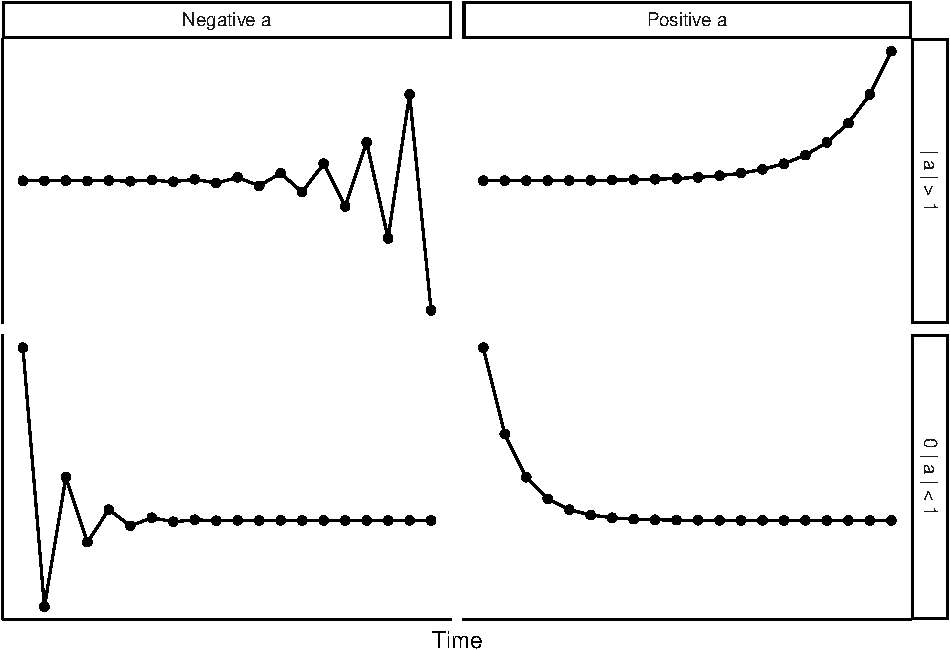
\includegraphics{figs/unnamed-chunk-9-1.pdf}
\caption{\label{fig:unnamed-chunk-9}dynamic equilibrium
fig\label{dynamics_plot}}
\end{figure}

\begin{figure}
\centering
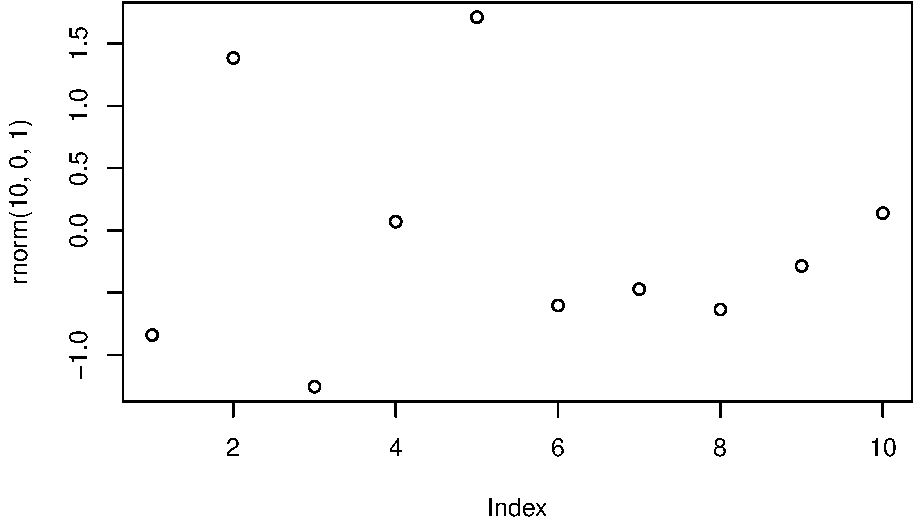
\includegraphics{figs/unnamed-chunk-10-1.pdf}
\caption{\label{fig:unnamed-chunk-10}this one will be a white noise process
and a random walk\label{noise}}
\end{figure}

\hypertarget{dynamic-modeling}{%
\subsection{Dynamic Modeling}\label{dynamic-modeling}}

We have introduced some fundemental concepts for dynamics. Memory,
constraints, random walks, equilibrium -- these are core ideas for
researchers to grapple with as they consider dynamic phenomenon. When
researchers then collect longitudinal data and estimate models (with
these ideas in mind) there are a host of challenges that must be
considered. In this section we are going to describe stationarity and
dynamic panel bias.

\hypertarget{stationarity}{%
\subsubsection{Stationarity}\label{stationarity}}

Stationarity is about the stability of the properties of a process.
Rachel's performance score across time is called a time-series -- it is
the trajectory of performance for a single unit (Rachel) over time. That
trajectory has properties: it has a mean and a variance. If the mean is
unstable then Rachel's performance either grows or decreases
unconditionally over time. If instead the mean is stable, then Rachel's
performance across time fluctuates but within the constraints of its
memory and bounds on the system. Almost all models used to estimate
coefficients in the organizational literature are stationary models that
assume the data they are modeling are realizations of a stationary
process. That is, they assume that the process they are trying to
estimate paramters for have properties at time \(t\) that are the same
as the properties at time \(t + 1\).

In simple terms, a stationary process has stable properties across time
-- data that demonstrate trend, growth, or random walk behavior are
(almost certainly) non-stationary. Here is the hard part: two
independent time-series will appear related if both are non-stationary
(kukljan; braun; granger). That is, if we measure Rachel's performance
and it is consistent with a random walk and we also measure rainfall at
Rachel's mother's house across the state and it demonstrates increasing
trend for the day, even though these two things are completely unrelated
we will more than likely find a relationship between them in a
regression-based analysis like those presented at the start of this
paper. There are many other papers that describe how to test for
stationarity (e.g., CITES), all we are trying to do here is convey how
important this notion is. Our literature is not paying attention to
random walks, we are not checking for memory, or seriel correlation, or
stationarity; we should be.

\hypertarget{dynamic-panel-bias}{%
\subsubsection{Dynamic Panel Bias}\label{dynamic-panel-bias}}

Another challenge for dynamic modeling is a congregation of effects
known as dynamic panel bias. First, in dynamics we pay attention to
memory, and our equations above took the form:

\begin{equation}
y_{t} = a y_{t-1} + e_{t}
\end{equation}

\noindent where the only change is that we replaced performance with a
generic \(y\). Again, these equations appropriately represent underlying
systems with memory, but when a researcher estimates a statistical model
and includes a lagged DV the errors become correlated with the
predictors and the well-known independence of errors assumption is
violated. This issue therefore has to do with estimating relationships
for a single unit when we want to incoporate lagged DVs.

The second issue arises when we are interested in relationships with a
multiple-unit sample across time. Almost all organizational studies are
multiple-unit -- they collect data on more than one participant. If the
people in the sample are not perfectly exchangeable, which means that I
can learn the same thing about performance and fatigue by studying
either Bob or Rachel, I lose no information by restricting my analysis
to one of them, then the parameter estimates are influenced by what is
known as unobserved heterogeneity. Unobserved heterogeneity represents
aggregate, stable individual differences. Rachel's fatigue over time may
look different from Bob's fatigue over time due to unmeasured individual
differences and states. These unacknowledged effects are responsible for
individual differences on fatigue so they need to be incorporated in
statistical models. We acknowledge them by incoporating unobserved
heterogeneity, again it is a term that is meant to represent all of the
unmeasured things that make Rachel's trajectory different from Bob's
trajectory.

In dynamic modeling unobserved heterogeneity must be handled
appropriately: if is is modeled as independent but in fact correlates
with the model predictors then ommitted variables bias is introduced
into the estimates, and if unobserved heterogeneity is ignored then
seriel correlation will be introduced into the errors.

Dynamic panel bias is the combined effect of these two biases. Lagged
DVs help us convey a dynamic process but they create estimation
problems, and unobserved heterogeneity must be accounted for.
Hierarchical linear models (or random-coefficient, multi level, random
effects) do not handle these biases appropriately (CITES).

\hypertarget{discussion---a-dynamic-perspective}{%
\section{Discussion - A Dynamic
Perspective}\label{discussion---a-dynamic-perspective}}

We opened this paper by talking about how researchers are beginning to
approach dynamics. We pointed to two frameworks -- growth and
relationships -- as example empirical research doing the hard work of
getting our thinking beyond static, cross-sectional relationships. They
were appropriate first steps toward dynamics given our field's history
with random coefficient models and recent introduction to growth curve
modeling, but there are many principles of dynamics outside the context
of a specific longitudinal model -- we broached them here. Taking a
dynamic perspective means focusing on memory, constraints, timescales,
reciprocal influence, initial conditions, and exploring an array of
satistical properties like serial correlation and stationarity.

\newpage

\hypertarget{references}{%
\section{References}\label{references}}

\setlength{\parindent}{-0.5in}
\setlength{\leftskip}{0.5in}

\hypertarget{refs}{}
\leavevmode\hypertarget{ref-dunford_is_2012}{}%
Dunford, B. B., Shipp, A. J., Boss, R. W., Angermeier, I., \& Boss, A.
D. (2012). Is burnout static or dynamic? A career transition perspective
of employee burnout trajectories. \emph{Journal of Applied Psychology},
\emph{97}(3), 637--650.
doi:\href{https://doi.org/http://dx.doi.org.proxy2.cl.msu.edu/10.1037/a0027060}{http://dx.doi.org.proxy2.cl.msu.edu/10.1037/a0027060}

\leavevmode\hypertarget{ref-gabriel_helping_2018}{}%
Gabriel, A. S., Koopman, J., Rosen, C. C., \& Johnson, R. E. (2018).
Helping others or helping oneself? An episodic examination of the
behavioral consequences of helping at work. \emph{Personnel Psychology},
\emph{71}(1), 85--107.

\leavevmode\hypertarget{ref-hulsheger_dawn_2016}{}%
Hülsheger, U. R. (2016). From dawn till dusk: Shedding light on the
recovery process by investigating daily change patterns in fatigue.
\emph{Journal of Applied Psychology}, \emph{101}(6), 905--914.
doi:\href{https://doi.org/http://dx.doi.org.proxy2.cl.msu.edu/10.1037/apl0000104}{http://dx.doi.org.proxy2.cl.msu.edu/10.1037/apl0000104}

\leavevmode\hypertarget{ref-johnson_good_2014}{}%
Johnson, R. E., Lanaj, K., \& Barnes, C. M. (2014). The good and bad of
being fair: Effects of procedural and interpersonal justice behaviors on
regulatory resources. \emph{Journal of Applied Psychology},
\emph{99}(4), 635.

\leavevmode\hypertarget{ref-koopman_integrating_2016}{}%
Koopman, J., Lanaj, K., \& Scott, B. A. (2016). Integrating the Bright
and Dark Sides of OCB: A Daily Investigation of the Benefits and Costs
of Helping Others. \emph{Academy of Management Journal}, \emph{59}(2),
414--435.
doi:\href{https://doi.org/10.5465/amj.2014.0262}{10.5465/amj.2014.0262}

\leavevmode\hypertarget{ref-liebovitch2010dynamics}{}%
Liebovitch, L. S., Vallacher, R. R., \& Michaels, J. (2010). Dynamics of
cooperation--competition interaction models. \emph{Peace and Conflict},
\emph{16}(2), 175--188.

\leavevmode\hypertarget{ref-mcelreath_statistical_2016}{}%
McElreath, R. (2016). \emph{Statistical Rethinking: A Bayesian Course
with Examples in R and Stan} (Vol. 122). CRC Press.

\leavevmode\hypertarget{ref-monge_theoretical_1990}{}%
Monge, P. R. (1990). Theoretical and analytical issues in studying
organizational processes. \emph{Organization Science}, \emph{1}(4),
406--430.

\leavevmode\hypertarget{ref-rosen_who_2016}{}%
Rosen, C. C., Koopman, J., Gabriel, A. S., \& Johnson, R. E. (2016). Who
strikes back? A daily investigation of when and why incivility begets
incivility. \emph{Journal of Applied Psychology}, \emph{101}(11), 1620.

\leavevmode\hypertarget{ref-vancouver_translating_2018}{}%
Vancouver, J. B., Wang, M., \& Li, X. (2018). Translating Informal
Theories Into Formal Theories: The Case of the Dynamic Computational
Model of the Integrated Model of Work Motivation. \emph{Organizational
Research Methods}, 109442811878030.
doi:\href{https://doi.org/10.1177/1094428118780308}{10.1177/1094428118780308}


\end{document}
